\documentclass[12pt]{article} % A4 paper

\usepackage[T1]{fontenc} % Use 8-bit encoding that has 256 glyphs
\usepackage[utf8]{inputenc}

\usepackage[spanish, es-tabla]{babel} % Selecciona el español para palabras introducidas automáticamente, p.ej. "septiembre" en la fecha y especifica que se use la palabra Tabla en vez de Cuadro
\usepackage{graphics,graphicx, float} %para incluir imágenes y colocarlas
\usepackage{booktabs}
\usepackage{xcolor}

\parskip=3pt

\usepackage[
    a4paper,
    left=2.8cm,
    right=2.7cm,
    top=2.5cm,
    bottom=2.5cm
]{geometry}

\par

%----------------------------------------------------------------------------------------
%	TÍTULO Y DATOS DEL ALUMNO
%----------------------------------------------------------------------------------------

\title{	

\vspace{-2.5cm}
\LARGE \textbf{Técnicas de los Sistemas Inteligentes} \\
\LARGE Práctica 2: Satisfacción de restricciones con MiniZinc \\[0.5em]
\large Curso 2021-2022 \par
\large Pedro Bedmar López - 75935296Z \\
\normalsize pedrobedmar@correo.ugr.es \par
\large Grado en Ingeniería Informática
\vspace{-7pt}
\rule{\textwidth}{0.4pt}
\vspace{-2cm}
}

\date{}

%----------------------------------------------------------------------------------------
% DOCUMENTO
%----------------------------------------------------------------------------------------

\begin{document}

\clearpage
\maketitle % Muestra el Título

\section{Problema de las monedas}
En este ejercicio se pretende resolver el problema de que dada una cantidad de dinero, se devuelve en monedas de 1, 2, 5, 10, 20 y 50 céntimos y en monedas de 1 y 2 euros.

\subsection{Apartado a)}
En este apartado calculamos cualquier solución válida, o sea, cualquier combinación de esas monedas que sume exactamente el importe introducido. Al no existir ninguna restricción aparte del uso de esas monedas específicas, el número de soluciones es muy alto y crece exponencialmente (como también lo hace el tiempo de ejecución).
% TODO: Crece exponencialmente el número de soluciones y el tiempo?

En la siguiente tabla se muestran los resultados de ejecución en 4 situaciones. La solución encontrada se expresa como un vector [c1,c2,c5,c10,c20,c50,e1,e2], donde cx representa la cantidad de monedas de x céntimos y ex la cantidad de monedas de x euros.

\begin{table}[H]
\centering
\begin{tabular}{@{}c|lll@{}}
\toprule
Importe &
    \multicolumn{1}{c}{\begin{tabular}[c]{@{}c@{}}Primera solución encontrada\\ y número de monedas de la misma\end{tabular}} &
    \multicolumn{1}{c}{\begin{tabular}[c]{@{}c@{}}Número total\\ de soluciones\end{tabular}} &
    \multicolumn{1}{c}{\begin{tabular}[c]{@{}c@{}}Runtime\\ (en segundos)\end{tabular}} \\ \midrule
0.17€ & {[}17,0,0,0,0,0,0,0{]} $\rightarrow$ 17 monedas   & 28     & 0.286  \\
1.43€ & {[}143,0,0,0,0,0,0,0{]} $\rightarrow$ 143 monedas & 17952  & 2.692  \\
2.35€ & {[}235,0,0,0,0,0,0,0{]} $\rightarrow$ 235 monedas & 150824 & 25.764 \\
4.99€ & {[}499,0,0,0,0,0,0,0{]} $\rightarrow$ 499 monedas & 6224452  & 2002 \\ \bottomrule
\end{tabular}
\caption{Resultados del apartado a) del problema de las monedas.}
\label{tab:my-table}
\end{table}

\subsection{Apartado b)}
En este caso, añadimos restricciones extra que impiden que con monedas de céntimo podamos representar un euro o más. Debido a esto el espacio de búsqueda se va a reducir y el tiempo de ejecución por tanto también disminuye. 

\begin{table}[H]
\centering
\begin{tabular}{@{}c|lll@{}}
\toprule
Importe &
    \multicolumn{1}{c}{\begin{tabular}[c]{@{}c@{}}Primera solución encontrada\\ y número de monedas de la misma\end{tabular}} &
    \multicolumn{1}{c}{\begin{tabular}[c]{@{}c@{}}Número total\\ de soluciones\end{tabular}} &
    \multicolumn{1}{c}{\begin{tabular}[c]{@{}c@{}}Runtime\\ (en segundos)\end{tabular}} \\ \midrule
0.17€ & {[}17,0,0,0,0,0,0,0{]} $\rightarrow$ 17 monedas  & 28    & 0.342 \\
1.43€ & {[}43,0,0,0,0,0,1,0{]} $\rightarrow$ 143 monedas & 284   & 0.311 \\
2.35€ & {[}35,0,0,0,0,0,2,0{]} $\rightarrow$ 235 monedas & 324   & 0.412 \\
4.99€ & {[}99,0,0,0,0,0,4,0{]} $\rightarrow$ 499 monedas & 13098 & 2.200 \\ \bottomrule
\end{tabular}
\caption{Resultados del apartado b) del problema de las monedas}
\label{tab:my-table}
\end{table}

\subsection{Apartado c)}
En este caso observamos que los tiempos de ejecución son menores o iguales que en el caso anterior. Esto se debe a que para problemas de optimización, MiniZinc no recorre todo el espacio de búsqueda, sino aquellas áreas donde es más probable encontrar la solución primero.
% TODO: es correcto?

% Please add the following required packages to your document preamble:
% \usepackage{booktabs}
\begin{table}[H]
    \centering
    \begin{tabular}{@{}c|ll@{}}
    \toprule
    Importe &
      \multicolumn{1}{c}{\begin{tabular}[c]{@{}c@{}}Solución óptima y número\\ de monedas de la misma\end{tabular}} &
      \multicolumn{1}{c}{\begin{tabular}[c]{@{}c@{}}Runtime\\ (en segundos)\end{tabular}} \\ \midrule
    0.17\texteuro  & {[}0,1,1,1,0,0,0,0{]} $\rightarrow$ 3 monedas & 0.283 \\
    1.43\texteuro  & {[}1,1,0,0,2,0,1,0{]} $\rightarrow$ 5 monedas & 0.327 \\
    2.35\texteuro  & {[}0,0,1,1,1,0,0,1{]} $\rightarrow$ 4 monedas & 0.338 \\
    4.99\texteuro  & {[}0,2,1,0,2,1,0,2{]} $\rightarrow$ 8 monedas & 0.376 \\ \bottomrule
    \end{tabular}
    \caption{Resultados del apartado c) del problema de las monedas}
    \label{tab:my-table}
    \end{table}

\subsection{Apartado d)}
\subsubsection*{¿Qué ocurriría si, usando la codificación (a) para encontrar todas las soluciones, el importe buscado es mucho mayor?} 
Ocurre que el espacio de búsqueda crece exponencialmente, y de la misma forma lo hace el tiempo de ejecución, por lo tanto llega un punto en el que el problema es inabarcable. 

\subsubsection*{¿Se podría encontrar alguna solución (usando la codificación de (a) o cualquier otra) de este problema con un importe del orden de los millones de euros? En caso afirmativo, ¿cuál podría ser una estrategia prometedora?}
Sí, una codificación donde únicamente existan monedas de un céntimo sería más eficiente y podría resolver el problema con tiempos de ejecución menores. Su coste computacional sería O(n).

Otra estrategia prometedora podría utilizar monedas de dos euros, dividiendo la cantidad millonaria entre esta cifra de forma iterativa, hasta llegar a un punto donde no pudiéramos dividir más por ser el cociente de la división menor a 1. En ese punto, completaríamos con el resto de monedas disponibles. De esta forma, la complejidad de tratar la cantidad millonaria se reduce en gran medida.
%TODO: Está correcto lo que acabo de explicar?

\section{Problema de los horarios}
Como se puede observar en las tablas inferiores, existen dos soluciones para este problema. La única diferencia entre ellas es el intercambio de las asignaturas en color rojo.

\begin{table}[H]
\centering
\begin{tabular}{c|ccccc}
\multicolumn{1}{l|}{} & L  & M  & X  & J  & V  \\ \hline
8-9                   & A4 & A4 & A8 & A5 & A5 \\
9-10                  & A4 & A4 & A8 & A5 & A5 \\
10-11                 & A9 & A7 & A6 & A2 & A6 \\
11-12                 & NA & NA & NA & NA & NA \\
12-13                 & A1 & A1 & A3 & A3 & \color{red}A2 \\
13-14                 & A1 & A1 & A3 & A3 & \color{red}A7
\end{tabular}
\caption{Solución 1 al problema de los horarios}
\label{tab:my-table}
\end{table}
\vspace{2pt}
\begin{table}[H]
\centering
\begin{tabular}{c|ccccc}
\multicolumn{1}{l|}{} & L  & M  & X  & J  & V  \\ \hline
8-9                   & A4 & A4 & A8 & A5 & A5 \\
9-10                  & A4 & A4 & A8 & A5 & A5 \\
10-11                 & A9 & A7 & A6 & A2 & A6 \\
11-12                 & NA & NA & NA & NA & NA \\
12-13                 & A1 & A1 & A3 & A3 & \color{red}A7 \\
13-14                 & A1 & A1 & A3 & A3 & \color{red}A2
\end{tabular}
\caption{Solución 2 al problema de los horarios}
\label{tab:my-table}
\end{table}

En mi caso, por cómo he representado el problema y por las restricciones que he empleado, no he obtenido soluciones simétricas. Un caso donde se me ocurre que podrían aparecer es utilizando identificadores distintos para cada recreo. En mi caso, los recreos siempre los fuerzo a tomar valor 0, pero si pudieran tomar valores diferentes para cada día (-1, -2, -3, -4 y -5, por ejemplo) aquí encontraríamos simetrías, soluciones que semánticamente significan lo mismo, pero que poseen valores diferentes. El recreo del lunes podría tomar valor -1 y el del martes -2, pero también podría ocurrir al revés, siendo las soluciones semánticamente idénticas.

Otra simetría aparecería si nuestra codificación diferenciara cada uno de los bloques lectivos de una misma asignatura. En ese caso, por ejemplo, las dos primeras horas del lunes y del martes se podrían intercambiar, dando lugar a dos soluciones semánticamente idénticas.

Como podemos observar, la estrategia para evitar simetrías consiste en hacer coincidir el dominio de las variables con su dominio semántico, de forma que la cardinalidad de ambos sea la misma.
% TODO: está esto bien?

\section{Problema lógico}
En este ejercicio solo existe una solución posible: el andaluz bebe agua y la cebra está en la casa verde.
% TODO: qué más poner en este ejercicio?

\section{Problema de la asignación de tareas}
Utilizando la primera versión del ejercicio, sin el cuarto trabajador de apoyo, el tiempo mínimo requerido para completar la construcción es de 12 días.

\begin{figure}[H] %con el [H] le obligamos a situar aquí la figura
    \centering
        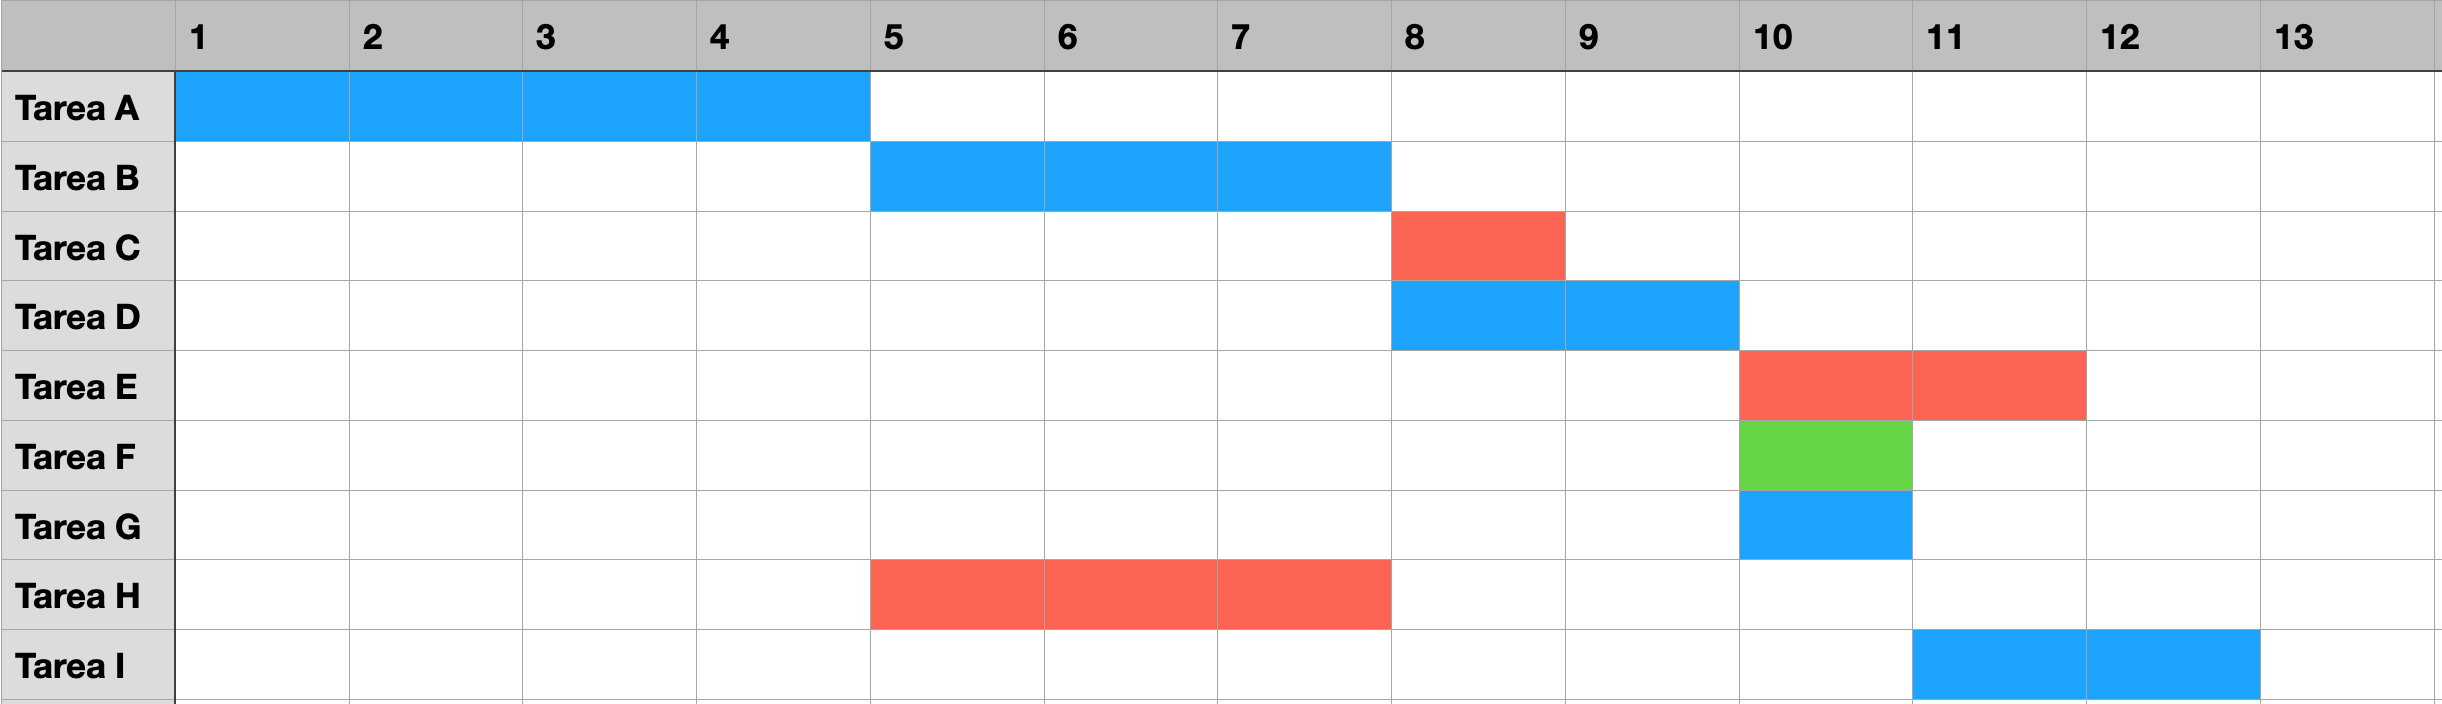
\includegraphics[scale=0.32]{gantt.png}
        \caption{Diagrama de Gantt de la solución sin el cuarto trabajador}
\end{figure}

\section{Problema del coloreado de grafos}
Al igual que ocurre en el problema 1a), este también crece de forma exponencial y se hace inabarcable. Se puede comprobar observando los tiempos de ejecución en la tabla inferior.
% TODO: el profesor espera aquí que hablemos de propagación unitaria?

\begin{table}[H]
\centering
\begin{tabular}{c|cc}
\multicolumn{1}{l|}{Tamaño del grafo} &
    \begin{tabular}[c]{@{}c@{}}Número de\\ colores mínimo\end{tabular} &
    \begin{tabular}[c]{@{}c@{}}Runtime\\ (en segundos)\end{tabular} \\ \hline
N=4, M=6   & 3 3 2    & 0.595 0.598 0.328 \\
N=6, M=15  & 5 5 4    & 0.522 0.533 0.606 \\
N=8, M=28  & 6 6 7    & 0.399 0.310 0.342 \\
N=10, M=45 & 8 8 8    & 0.942 0.853 0.678 \\
N=12, M=66 & 10 8 9   & 38.7 1.106 3.840  \\
N=14, M=91 & 11 11 12 & 1365 410 5216    
\end{tabular}
\caption{Valores medios de ejecución del problema de coloreado de grafos}
\label{tab:my-table}
\end{table}


\end{document}